\begin{frame}{Tijd om te installeren!}
    \begin{columns}
        \begin{column}{0.4\textwidth}
            \tiny
            % \begin{enumerate}[label={\arabic*)}]
            %     \item Installeer MiKTeX (Windows), MacTeX (Mac) of TeX Live (Linux)
            %     \item Update packages (Bij MiKTeX: `MiKTeX Console')
            %     \item Enkel nodig op Windows: Installeer Perl (https://strawberryperl.com)
            %         % (of ga naar de
            %         % gedetailleerde instructies voor alternatief)
            %     \item Installeer VS Code
            %     \item Voeg `LaTeX Workshop' extensie toe in VS Code
            %     \item Sla bestand op met .tex-extensie, en compileer in VS Code
            %     %\item Compileer een simpel bestand in VS Code
            % \end{enumerate}

            Installatie is gesplitst in gespecialiseerde onderdelen. \textbf{Allemaal
            nodig!}
            \medskip

            Voor Windows:
            \begin{enumerate}[label=\arabic*), itemsep=0pt]
                \item MiKTeX: \url{https://miktex.org/download}
                \item Perl: \url{https://strawberryperl.com}
                \item Visual Studio Code: \url{https://code.visualstudio.com}
            \end{enumerate}

            Voor Mac:
            \begin{enumerate}[label=\arabic*), itemsep=0pt]
                \item MiKTeX: \url{https://miktex.org/download}
                \item Visual Studio Code: \url{https://code.visualstudio.com}
            \end{enumerate}

            Voor Linux:
            \begin{enumerate}[label=\arabic*), itemsep=0pt]
                \item TeX Live: \texttt{sudo apt install texlive}
                \item Visual Studio Code: \url{https://code.visualstudio.com}
            \end{enumerate}

            Als je Linux gebruikt en een GUI wil, installeer dan MiKTeX i.p.v. TeX Live.

            % \bigskip

            % Klaar? Ga naar de volgende webpagina en probeer wat snippets en
            % shortcuts ervan uit:
            
            % \url{https://github.com/James-Yu/LaTeX-Workshop/wiki/Snippets}
            %en probeer wat snippets en shortcuts uit
        \end{column}
        \begin{column}{0.6\textwidth}
            \tiny
            %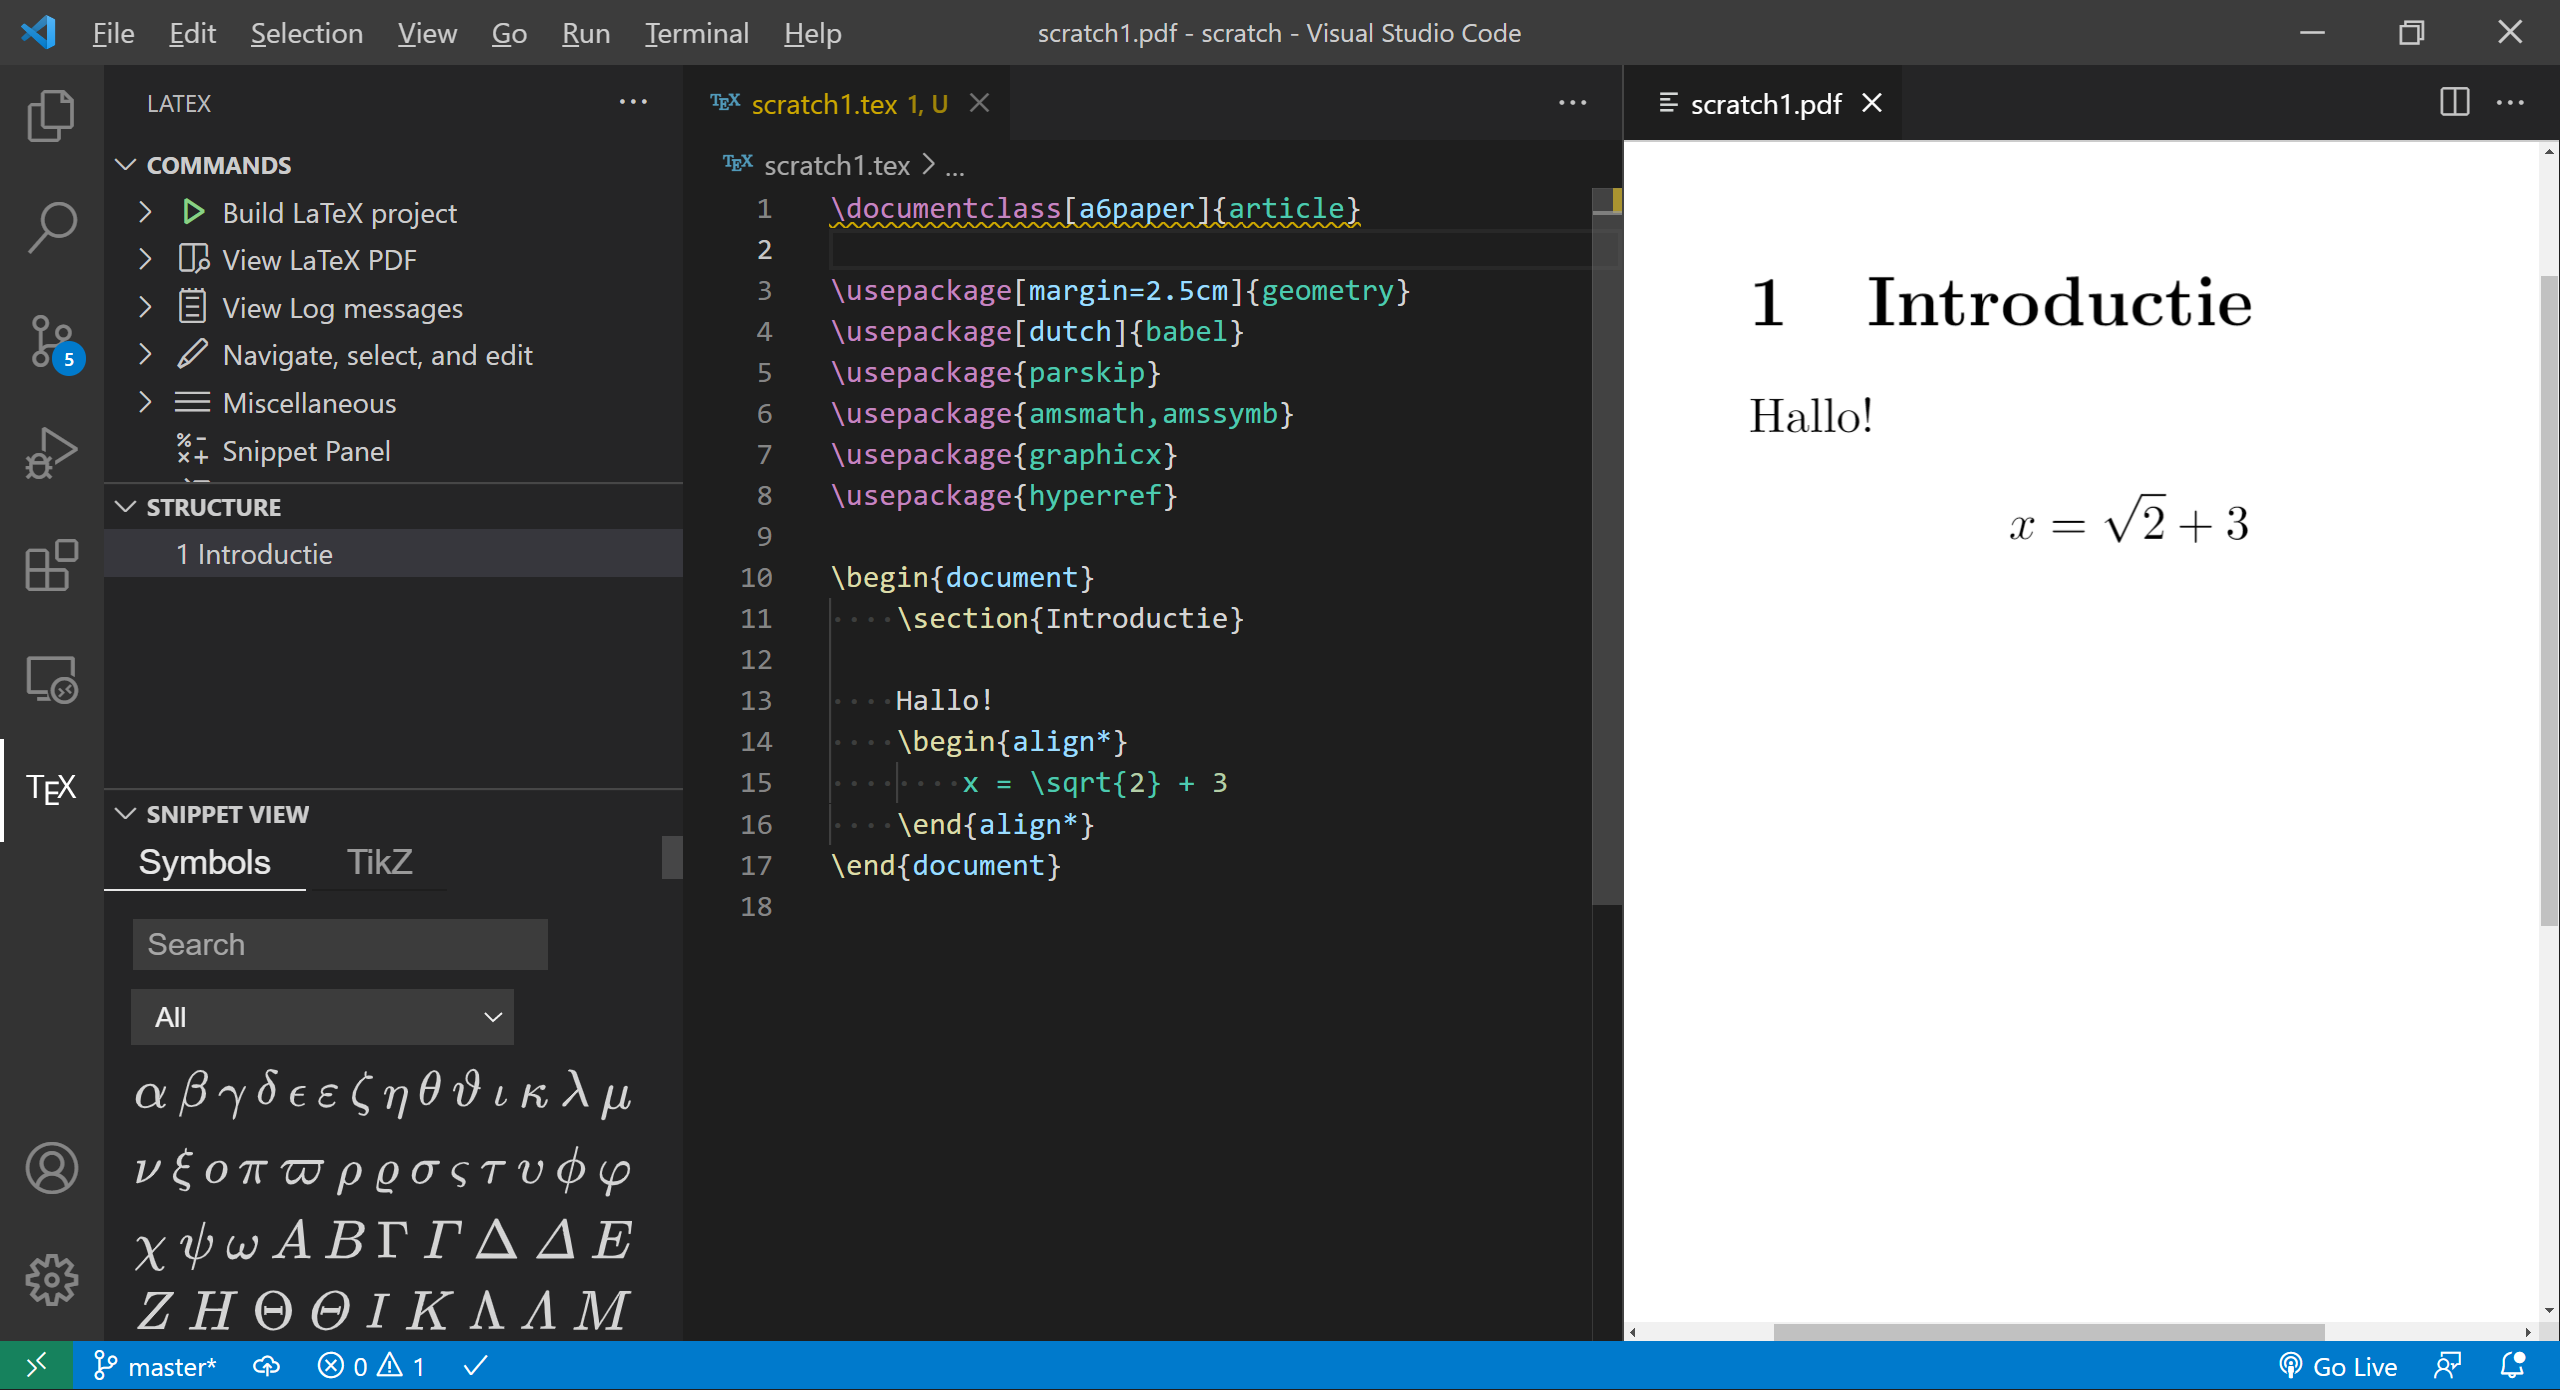
\includegraphics[width=\linewidth,height=0.8\textheight,keepaspectratio]{assets/VisualStudioCodeDemo.png}
            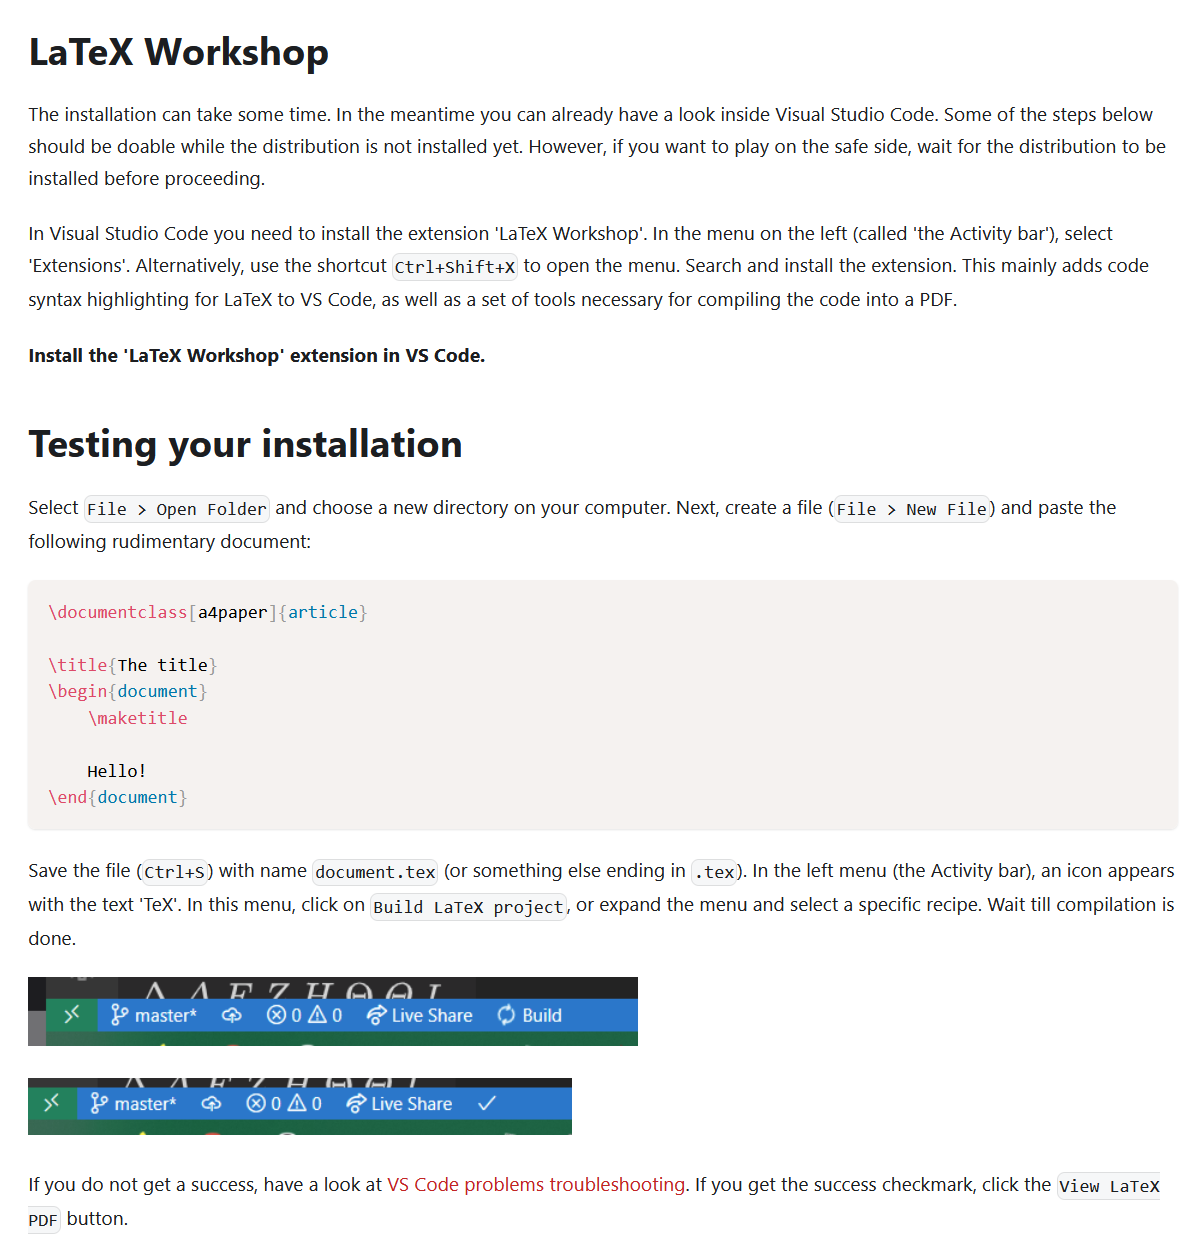
\includegraphics[width=\linewidth,height=0.8\textheight,keepaspectratio]{assets/installLaTeXWorkshop.png}

            {\tiny
            Gedetailleerde instructies:
            \href{https://vkuhlmann.com/latex/installation}{\nolinkurl{vkuhlmann.com/latex/installation}}}


            % Klaar? Ga naar de volgende webpagina en probeer wat snippets en
            % shortcuts ervan uit:
            
            % \url{https://github.com/James-Yu/LaTeX-Workshop/wiki/Snippets}
            %en probeer wat snippets en shortcuts uit
        \end{column}
    \end{columns}
\end{frame}